% !TEX program = xelatex
\documentclass{article}
\usepackage[utf8]{inputenc}
\usepackage{amsmath}
\usepackage{relsize}
\usepackage{amssymb}
\usepackage{mathabx}
\usepackage{amsthm}
\usepackage{graphicx}
\usepackage[usenames,dvipsnames]{xcolor}
\newcommand{\kacper}[1]{ \bf  { \color{Orchid}{Kc: #1}}  }

\newtheorem{definition}{Definition}
\newtheorem{lemma}{Lemma}
\newtheorem{Theorem}{Theorem}
\newtheorem{example}{Example}
\newtheorem{statement}{Statement}
\newtheorem{corollary}{Corollary}
\newtheorem{test}{Test}
\newtheorem{proposition}{Proposition}

\newtheorem*{remark}{Remark}
\newenvironment{claim}[1]{\par\noindent\underline{Claim:}\space#1}{}
\newenvironment{claimproof}[1]{\par\noindent\underline{Proof:}\space#1}{\hfill $\blacksquare$}

\title{Testing MCMC methods convergance}
\author{KC,AG}
\date{}



\begin{document}

\maketitle

Let $g(x,y)$ be a characteristic, analytic kernel. Let $p$ be a probability measure on $R^d$; suppose it has a density which logarithm exists, and is differentiable. Consider the following transform of $R^d$ valued random variable $X$
\begin{align}
 \mu_p(y) = E  \nabla \log p(X) g(X,y) - E \nabla g(X,y)
\end{align}
this transform is closely connected to Stein method and kernel mean embedding.

\begin{statement}
 If $X$ is distributed according to $p$ then the function  $\mu_p(y)$ is identically equal to zero  
\end{statement}
\begin{proof}
 For a fixed $y$ this is consequence of Stein method with as described in NIPS paper.   
\end{proof}

\begin{statement}
 If $X$ is not distributed according to $p$, but has a density, then $\mu_p(y)$ is different form zero almost everywhere. 
\end{statement}
\begin{proof}
 Suppose $X$ is distributed according to density $p'$, then

\begin{align}
\mu_p(y) =& \int_{R^d} ( \nabla \log p(x) g(x,y) -  \nabla g(x,y)) p'(x) dx \\
          & \int_{R^d} g(x,y) \frac{ p'(x)}{p(x)} \nabla p(x) - \nabla g(x,y) p'(x)  
\end{align}
Integration by parts and funshows that for all partial derivatives 
\begin{align}
0 = \int_{R} \frac{ \partial g(x,y)p'(x)} { \partial x_i } dx_i
\end{align}
\begin{align} 
 \int_{R} \frac{ \partial g(x,y) } { \partial x_i } p'(x) d x_i =
 -\int_{R} \frac{ \partial p(x) } { \partial x_i } g(x,y) d x_i 
\end{align}
So
\begin{align}
\mu_p(y) =& \int_{R^d} g(x,y) \frac{ p'(x)}{p(x)} \nabla p(x) -  g(x,y) \nabla p'(x)  \\
	 =& \int_{R^d} g(x,y) \left( \frac{ p'(x)}{p(x) } \nabla p(x) -  \nabla p'(x) \right)
\end{align}
 We would like to say that $t(x) = \frac{ p'(x)}{p(x) } \nabla p(x) -  \nabla p'(x)$  is kind of bounded and invoke the argument that $\mu_p$ is analytic, but first we need to prove that $t(x)$ is non-zero. 
 It is sufficent to see that $t(x) =0$ imples that $\nabla [ \log( p(x)) - \log( p'(x)) ]=0$, which imples that $p(x) = p'(x)e^C$. Since both $p$ and $p'$ are probability measures,  $C$ must be equal to 0.
 
 $\mu_p$ lives in the $RKHS$ associated with kernel $g$. Indeed if the integaral exists 
 \[
  \int f(x) t(x) 
 \]
 then there exist an element $\mu_t$, such that $<\mu_t, f>$ is equal to above integral and in addition to that 
 \[
  \mu_t(t) = < \mu_t, k(t,\cdot)> = \int k(t,x) t(x) = \mu_p(t). 
 \]
The sufficent consition for $\int f(x) t(x)$ to exist is that 
\[
 \int <f, k(x,)> t(x) = < f, \int k(x,) t(x) > 
\]
$\int k(x,) t(x) $ exists and this one is easilly verifiable for popular kernel (e.g. exists for expontial families and gausian kernel). By the lemm form our previous paper we see that $\mu_p(t)$ is  analytic. 
\end{proof}

\paragraph{Temporal dependence -- not an issue}
There are several ways to deal with temporal dependence, all of which, to our knowledge, work only asymptotically. Options include estimating auto-covariances, performing bootstrap or thinning. The last one, usually avoided in time-series analysis due to it's wasteful approach to data, is quite feasible in this application. It is also equally or less computationally complex then other options (potentially less noisy then estimating the auto covariance).      

It's obvious, but needs to show formally, that distribution of the test statistic under the null hypothesis, as $n$ approaches infinity, is as if we had used IID data. This is proved in appendix.

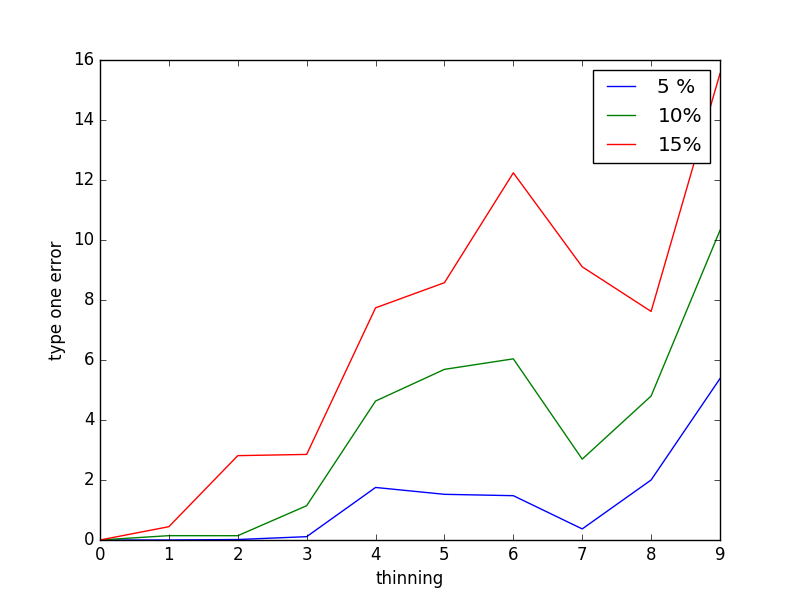
\includegraphics[width=0.8\textwidth]{type1.png}

\section{Sample selection}
so far we've agnostic the the problem of selecting sample on which to perform a test. In this section we propose a procedure that returns a sample for which it can not be rejcted that it was generated from null distribution. We will proceed as in Heidelberger-Welch (Estimating convergence of Markov chain
Monte Carlo simulations) method -- firts, the whole output sequance is is tested with our statistic to see if output can be assumed to to be disitbuted as as a Brownian Bridge. If the null hypothesis is rejected, the test is repeted with 10 \%, 20\%, ...of the chain discarded. The procedure of dicaring is continued untill some part of the chain is considered to be stationary or 50 \% of the chain has been discarded, in which case chain has to be run longer. 

\paragraph{type One-error}
We will use simple Bonferroni correction to deal with type one error. Tests level must be adjusted, so that they sum up to $\alpha$. Any scheme can be used, we use $\frac{1}{x^2}$ since we believe (am I turning  Bayesian? ) that chain converge fast.   

\paragraph{Type two}
Type two is somehow more complicated, but also quite important. In general (this is my intuition from finite state markov chains and AR processes ) chain does not converge to stationary distribution in any number of finite steps, unless it has started for the stationary distribution itself. As usually in testing, one has no finite sample control over type two error and hope must be lost. We can however infer what misspecified log probability would have given similar results on this sample. This can be done by perturbing log probability in some direction and calculating the statistic on our sample. The magnitude of perturbation will show which models appear to be indistinguishable (now talk about parametres inference and that its even more difficult )    

















\end{document}


